\documentclass[12pt]{article}
\usepackage{cover} % contains cover-page definitions
\usepackage{xcolor}
\usepackage{tikz}
\usetikzlibrary{positioning, arrows.meta, shapes.geometric, fit, backgrounds}
\usepackage{subcaption}
\usepackage{float}

% Highlight unfinished text so it cannot be missed. Delete every \todo{} before submitting.
\newcommand{\todo}[1]{\textcolor{red}{\textbf{[TODO: #1]}}}

\begin{document}

% --- FILL THIS OUT ---
% Working title (suggested 2026-10-31; the final wording is for you and your advisor to decide).
\title{Voice-Driven, Safety-Guarded Pick-and-Place with a Local LLM Planner and Self-Improving Grasp Selection on a Kinova Gen3 Arm}
\author{Shashwat Shah}
\degreemonth{\todo{month}}
\degreeyear{\todo{year}}
\chair{Prof.\ Mingyu Cai}
\othermembers{\todo{2nd committee member}}
\numberofmembers{2}

% --- Cover Page ---
\makecover
\newpage


% --- Abstract ---
\thispagestyle{empty}
\begin{abstract}

Spoken commands are a natural way to instruct a robot arm, but connecting speech to safe, reliable manipulation on real hardware is hard: language models can produce plans that are wrong or unsafe, cameras drift, and grasps fail in ways a planner cannot foresee.
This project builds a complete voice-to-manipulation system for a Kinova Gen3 7-DOF arm with a Robotiq 2F-140 gripper, in which a command such as ``pick up the white cup and put it near the robot base'' is transcribed offline, turned into a plan by a deterministic command grammar backed by a locally run language model (Qwen2.5-7B), grounded in a live scene built from three depth cameras and the wrist camera, and executed through MoveIt~2.
Nothing in the pipeline depends on a cloud service.

The contribution is less any single component than the engineering that makes the chain dependable: a multi-camera scene graph with occlusion-aware colour recognition, a board-based calibration procedure with independent checks and an automatic warning when two cameras disagree, a whole-arm safety layer that fails closed, a human-style side grasp learned from a hand-guided demonstration, and a grasp chooser that learns success rates by position on the table from its own outcome log.
In live development trials (132 recorded picks over three weeks, which include faults fixed since) 88 picks succeeded; a controlled evaluation with fixed protocols is still in progress and is described in Section~\ref{sec:results}.

\end{abstract}

\pagebreak
{\newpage\renewcommand{\thepage}{\arabic{page}}\setcounter{page}{1}}

% --- Main Content ---

\section{Introduction}

A person at a bench should be able to say ``give me the blue cup'' and have a robot arm do it. Large language models (LLMs) make the language side of this look easy, but the physical side is not: a plan that names an object only helps if the cameras place that object correctly in the robot's frame, if the arm can reach it without touching the table or itself, and if the grasp holds. Each of these steps fails in practice, and the failures compound.

This project addresses the whole chain on one real robot rather than one link in isolation. The system has four parts: (i) \emph{speech and planning}, where a command is transcribed offline and converted into a short list of primitive actions; (ii) \emph{perception}, where three RealSense depth cameras and the wrist camera are fused into one scene of named, coloured, positioned objects; (iii) \emph{execution}, where an arm controller chooses how to grasp, checks every motion against safety limits, and drives MoveIt~2; and (iv) \emph{monitoring}, a web dashboard for the cameras, the arm, calibration and the system's health.

\paragraph{Contributions.}
\begin{itemize}
  \item A fully local voice-to-manipulation pipeline (offline speech recognition, a command grammar with a local LLM fallback, MoveIt~2 execution) on a 7-DOF arm.
  \item A multi-camera scene graph with per-camera weighting, a correction for the fact that depth cameras measure an object's near surface, and colour recognition that is robust to occlusion and lighting (Section~\ref{sec:perception}).
  \item A calibration procedure for static cameras built on a wrist-anchored ChArUco board with independent verification against the arm itself, and a run-time health check that detects a moved camera (Section~\ref{sec:calibration}).
  \item A grasp chooser that selects between top-down and side grasps from the scene and learns position-dependent success rates from its own outcome log (Section~\ref{sec:grasp}).
  \item A safety layer that guards the whole arm, not only the gripper, and refuses to move when its assumptions cannot be confirmed (Section~\ref{sec:safety}).
\end{itemize}

\section{Related Work}

\paragraph{Language-conditioned manipulation.}
SayCan~\cite{ahn2022saycan} grounds an LLM's proposals in learned affordance values so that only feasible skills are chosen; Code as Policies~\cite{liang2023codeaspolicies} has the model write programs that call perception and control primitives; Inner Monologue~\cite{huang2022innermonologue} feeds scene and success feedback back into the model. End-to-end vision-language-action models such as RT-2~\cite{brohan2023rt2} go further and output actions directly. These systems rely on large hosted models and on robot data collected at scale. This project takes the opposite design point: a small local model (Qwen2.5~\cite{qwen2024qwen25}) behind a deterministic grammar, with a fixed action vocabulary and a safety layer that can veto any plan, so that behaviour on a single lab robot is predictable and auditable.

\paragraph{Speech and perception.}
Offline speech recognition uses Whisper~\cite{radford2023whisper}. Object detection uses YOLOv8~\cite{jocher2023yolov8} with OpenCV~\cite{bradski2000opencv} for image processing. The contribution here is not the detectors but how their outputs are fused across cameras and made reliable enough to plan against (Section~\ref{sec:perception}).

\paragraph{Motion planning and software.}
Motion planning uses MoveIt~\cite{coleman2014moveit} with OMPL~\cite{sucan2012ompl} on ROS~2~\cite{macenski2022ros2}. Planner output is passed through a time-parameterisation and then through our own checks (Section~\ref{sec:safety}), because a collision-free plan for the modelled robot is not the same as a safe one for the real table.

\paragraph{Calibration.}
Locating a fixed camera in the robot's frame is a hand-eye calibration problem~\cite{tsai1989handeye,park1994handeye}; fiducial boards such as ArUco/ChArUco~\cite{garridojurado2014aruco} provide the pose measurements. We use the same mathematics but add independent checks against the arm and the table, because a self-consistent solution can still be wrong (Section~\ref{sec:calibration}).

\paragraph{Grasping.}
Learned grasp planners such as Dex-Net~\cite{mahler2017dexnet} predict grasp quality from depth. We instead use a small set of hand-designed grasp families (top-down, side, leaned) and learn only \emph{which family works where}, from the robot's own outcomes, which needs far less data.

\section{Methodology}
\label{sec:method}

\subsection{System overview}

Figure~\ref{fig:pipeline} shows the pipeline. A microphone feeds an offline Whisper transcriber. The text goes first to a command grammar that recognises the common commands (pick, put, place next to, near the base, aside, colour-qualified objects) and builds the plan directly; anything it does not recognise is planned by the local LLM, which is told the available actions, the workspace bounds and the current scene. Plans are lists of primitives (\texttt{pick}, \texttt{place}, \texttt{move\_to}, \texttt{go\_home}, gripper open/close). The arm controller executes them; it alone talks to MoveIt~2 and the gripper.

\begin{figure}[t]
\centering
\resizebox{\linewidth}{!}{%
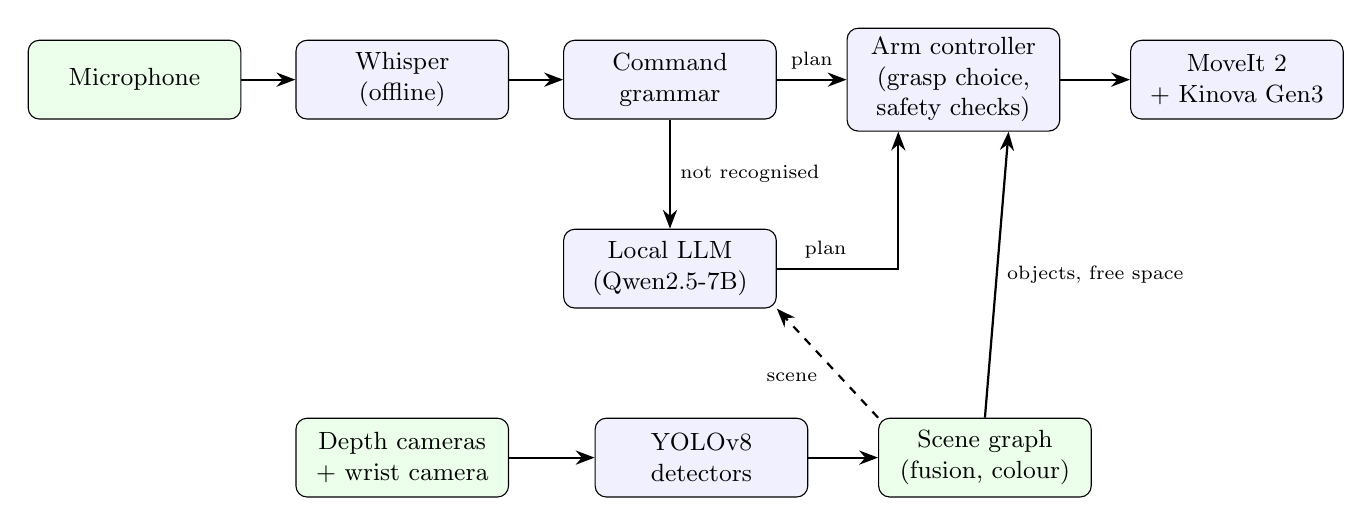
\begin{tikzpicture}[
  box/.style={draw, rounded corners, align=center, minimum height=10mm, minimum width=27mm, font=\small, fill=blue!6},
  io/.style={draw, rounded corners, align=center, minimum height=10mm, minimum width=27mm, font=\small, fill=green!8},
  arr/.style={-{Stealth[length=2.4mm]}, thick}
]
  % top row: speech -> plan -> robot
  \node[io]  (mic)   at (0,0)    {Microphone};
  \node[box] (asr)   at (3.4,0)  {Whisper\\(offline)};
  \node[box] (gram)  at (6.8,0)  {Command\\grammar};
  \node[box] (ctrl)  at (10.4,0) {Arm controller\\(grasp choice,\\safety checks)};
  \node[box] (moveit) at (14.0,0) {MoveIt 2\\+ Kinova Gen3};
  % middle: fallback planner
  \node[box] (llm)   at (6.8,-2.4) {Local LLM\\(Qwen2.5-7B)};
  % bottom row: perception
  \node[io]  (cams)  at (3.4,-4.8)  {Depth cameras\\+ wrist camera};
  \node[box] (yolo)  at (7.2,-4.8)  {YOLOv8\\detectors};
  \node[io]  (scene) at (10.8,-4.8) {Scene graph\\(fusion, colour)};

  \draw[arr] (mic) -- (asr);
  \draw[arr] (asr) -- (gram);
  \draw[arr] (gram) -- node[above, font=\scriptsize]{plan} (ctrl);
  \draw[arr] (ctrl) -- (moveit);
  \draw[arr] (gram) -- node[right, font=\scriptsize]{not recognised} (llm);
  \draw[arr] (llm.east) -| node[above, font=\scriptsize, pos=0.2]{plan} ([xshift=-7mm]ctrl.south);
  \draw[arr] (cams) -- (yolo);
  \draw[arr] (yolo) -- (scene);
  \draw[arr] (scene.north) -- node[right, font=\scriptsize]{objects, free space} ([xshift=7mm]ctrl.south);
  \draw[arr, dashed] (scene.north west) -- node[below left, font=\scriptsize, pos=0.5]{scene} (llm.south east);
\end{tikzpicture}}
\caption{Pipeline. Speech is transcribed offline and planned by a deterministic grammar, with a local LLM as fallback. Both are grounded in the same scene graph, built from the detectors on three static cameras and the wrist camera. The arm controller is the only component that commands the robot.}
\label{fig:pipeline}
\end{figure}

\subsection{Perception and the scene graph}
\label{sec:perception}

\paragraph{Fusion.}
Each camera reports detections with a 3D point in its own frame, transformed into the robot base frame using its calibration. For each tracked object the scene keeps every camera's latest reading and forms the weighted mean
\begin{equation}
  \hat{\mathbf p} = \frac{\sum_k w_k \mathbf p_k}{\sum_k w_k}, \qquad w_k = c_k\, s_k,
\end{equation}
where $c_k$ is the detection confidence and $s_k$ a per-camera reliability (RS1 and RS2 $1.0$, the noisier RS3 $0.3$, the wrist $0.4$). The published position moves a fraction $\alpha=0.35$ towards $\hat{\mathbf p}$ per message, and jumps to it when it differs by more than $6$\,cm (the object was moved). Before this per-camera scheme the published position followed whichever camera spoke last, so the map ``danced''.

\paragraph{Surface versus centre.}
A depth camera measures the \emph{near surface} of an object, but the arm needs its centre. Comparing against the wrist camera showed each static camera's error lies along its own line of sight, towards itself. The scene graph therefore moves a static-camera point away from the camera by the object's radius $r$ in the horizontal plane:
\begin{equation}
  \mathbf p_c = \mathbf p_s + r\,\frac{(\mathbf p_s-\mathbf o)_{xy}}{\lVert(\mathbf p_s-\mathbf o)_{xy}\rVert},
\end{equation}
with $\mathbf o$ the camera position. After this correction the fused scene agreed with the wrist camera to within about $0.8$--$3.5$\,cm on the objects tested.

\paragraph{Colour.}
Colour-qualified commands (``the white cup'') require a colour per object. The classifier looks at an ellipse inside each detection box, removes the table's own red-brown, and names the commonest hue if enough pixels are strongly saturated (median saturation of at least 165 on the 0--255 scale), otherwise a neutral (white, grey, black) from brightness. Two further measures were needed after live failures. \emph{Occlusion:} pixels inside the box of a nearer detection are excluded, because a white cup standing behind a teal one was read as blue by the side camera in every frame. \emph{Voting:} each camera keeps its own fading vote; the published colour comes from the cameras' \emph{normalised} votes weighted by reliability, so a camera that reports twice as often does not outvote the others, and a new colour must win ten evaluations in a row before the published one changes.

\subsection{Calibration and its verification}
\label{sec:calibration}

Static cameras are located with a ChArUco board seen simultaneously by the wrist camera and the camera being calibrated. With the arm's forward kinematics giving $T_{\text{base,wrist}}$,
\begin{equation}
  T_{\text{base,cam}} = T_{\text{base,wrist}}\; T_{\text{wrist,board}}\; T_{\text{cam,board}}^{-1}.
\end{equation}
Several captures (different board places and arm poses) are combined with outlier rejection. Because a single capture of a distant camera is noisy and a self-consistent result can still be biased, each candidate is checked independently of the board before it is installed:
\begin{itemize}
  \item \textbf{Table levelling.} The measured table plane (height recorded with the gripper pads) fixes the camera's height and tilt.
  \item \textbf{Arm as a ruler.} Points along the arm's skeleton, known exactly from the joint angles, are projected into the depth image; a well-placed camera shows a constant offset (about one link radius, $5.5$\,cm) with a small spread. This detects the error along the viewing direction that the board cannot reveal.
  \item \textbf{Cross-checks.} A second, board-free method (clicking known arm landmarks in the image) and the agreement of different cameras on the same objects.
\end{itemize}
At run time the scene graph records how far apart each pair of static cameras places the same object; when the median gap stays above $7$\,cm for two minutes the dashboard raises a warning that a camera has probably moved.

\subsection{Grasp selection and learning}
\label{sec:grasp}

Three grasp families are available. A \emph{top-down} grasp approaches vertically. A \emph{side} grasp copies a hand-guided demonstration: the tool is held $5.3^\circ$ below horizontal, the pads close just under the rim of a cup, and the approach azimuth can be rotated in $45^\circ$ steps to find a direction that is free of neighbours and reachable (Figure~\ref{fig:demo}). A \emph{leaned} grasp tilts the tool from vertical. For each candidate the chooser checks the footprint of the open fingers and wrist against neighbouring objects, checks inverse kinematics along the whole approach, and ranks the options.

\begin{figure}[t]
\centering
\begin{subfigure}{0.48\linewidth}
  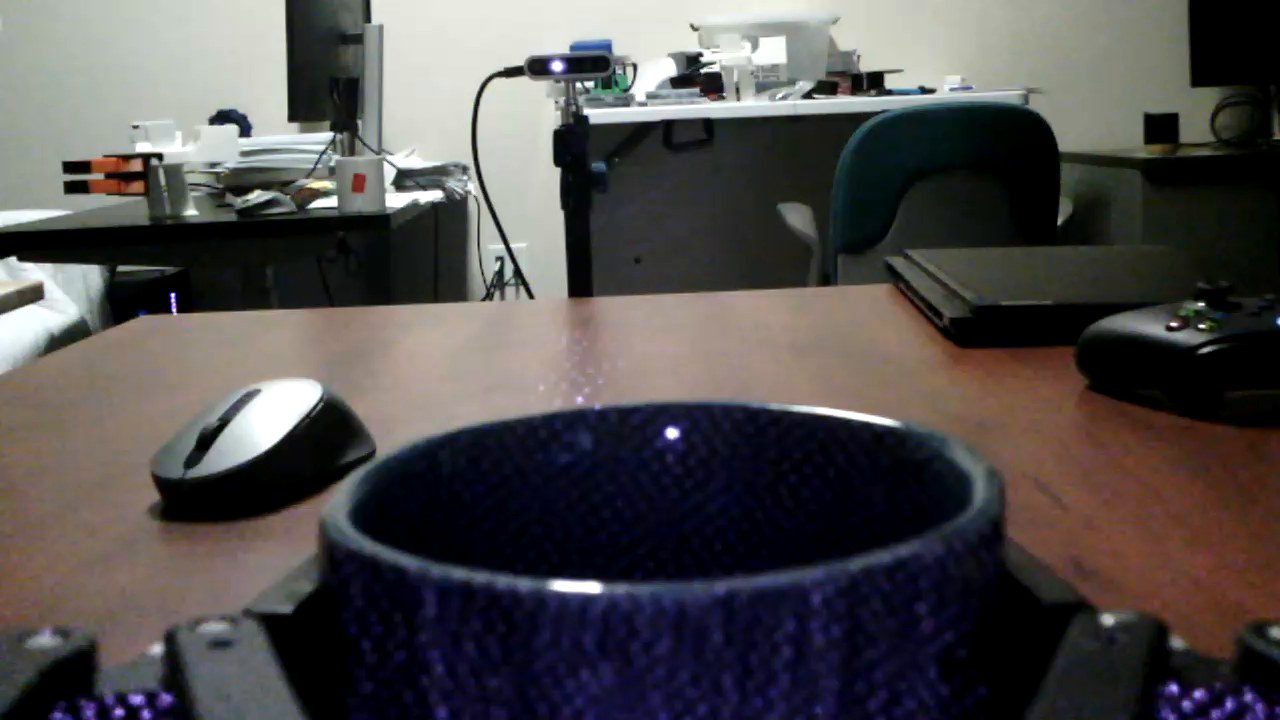
\includegraphics[width=\linewidth]{figures/side_grasp_wrist.jpg}
  \caption{Wrist camera.}
\end{subfigure}\hfill
\begin{subfigure}{0.48\linewidth}
  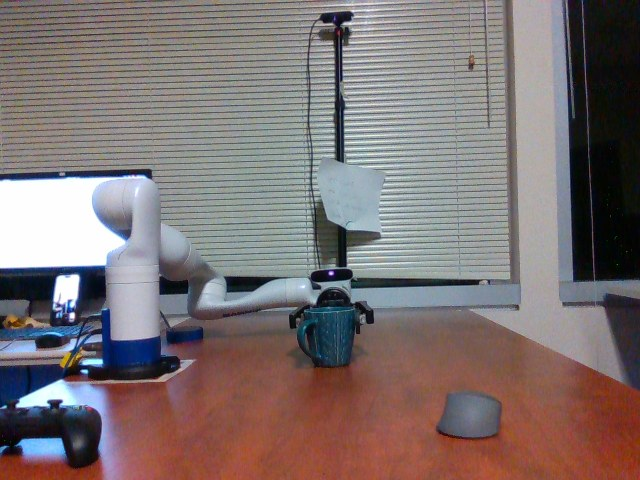
\includegraphics[width=\linewidth]{figures/side_grasp_rs2.jpg}
  \caption{Side camera (RS2).}
\end{subfigure}
\caption{The hand-guided demonstration the side grasp copies (2026-10-26): pads across the cup just under the rim, tool nearly horizontal.}
\label{fig:demo}
\end{figure}

\paragraph{Learning from outcomes.}
Every pick is logged with its object, position, method and result. For a method the success rate near a point $\mathbf x$ is a distance-weighted average that falls back to the method's overall rate where there is little local data:
\begin{equation}
  \hat p(\mathbf x)=\frac{\sum_i w_i\,\mathrm{ok}_i + m\,\bar p}{\sum_i w_i + m},\quad
  w_i=\exp\!\Big(-\frac{\lVert \mathbf x-\mathbf x_i\rVert^2}{2\sigma^2}\Big),\quad
  \bar p=\frac{s+1}{n+2},
\end{equation}
with $\sigma=0.10$\,m, $m=2$ pseudo-trials, and $s$ successes in $n$ trials overall. The method's score is scaled by $\hat p/0.5$ clipped to $[0.4,1.5]$. The side grasp is allowed inside a small proven zone and within $12$\,cm of any place where it has worked with local rate of at least $0.5$; a place whose local rate falls below $0.35$ is blocked for the method. The dashboard draws this map for inspection.

\subsection{Safety}
\label{sec:safety}

Every motion passes checks the planner does not know about. The flange and every arm link that can reach the table (not only the gripper) must stay above a floor tied to the recorded table height, orientation-aware for a horizontal tool; the fingers and wrist must stay in front of a rear limit; long swings are refused if their planned duration exceeds a gate; and the table and rear wall are re-applied to MoveIt's planning scene before every plan, with the plan refused if that cannot be confirmed (the system \emph{fails closed}). Fixed objects such as a coffee machine are declared in a configuration file; detections inside their footprint are dropped, and the arm treats them as tall obstacles. A held-object record survives restarts, and a gripper that is half closed with nothing in it is opened automatically. Jogging by hand uses the same checks.

\section{Results and Evaluation}
\label{sec:results}

\paragraph{Status of the evaluation.}
The results below come from the system's own logs during development (8--30 October 2026), together with measurements taken during calibration. They are \emph{not} a controlled experiment: the code changed during this period and several faults were fixed along the way, so early numbers understate the current system. A controlled evaluation is planned (below) and its table is left empty on purpose.

\subsection{Pick outcomes from the live log}

\begin{table}[H]
\centering
\caption{Live picks recorded in the outcome log, 8--30 October 2026 (development period).}
\label{tab:picks}
\begin{tabular}{llrrr}
\toprule
Object & Method & Picks & Successful & Rate \\
\midrule
Cup    & top  & 56 & 42 & 75\% \\
Cup    & side & 17 & 10 & 59\% \\
Mouse  & top  & 47 & 28 & 60\% \\
Bottle & top  &  9 &  7 & 78\% \\
Bowl, vase & top & 3 & 1 & --- \\
\midrule
All    &      & 132 & 88 & 67\% \\
\bottomrule
\end{tabular}
\end{table}

Over the same period the log holds 207 live commands, 139 of which completed (67\%), and 85 of 106 placements succeeded (80\%). A successful pick took a median of 26.5\,s. The most common failed steps were checking the grip (10), the final descent (8), the hover above the object (8) and the lift (7), followed by the finger-clearance check against neighbours (6) and turning the fingers away from a cup handle (3). The side grasp, which is the newest method, has the lowest rate so far; most of its failures were found and fixed in the first live sessions (for example a wrist flip in straight-line planning and a standoff distance that was too short).

\subsection{Calibration}

\begin{table}[H]
\centering
\caption{Calibration measurements, 29--30 October 2026.}
\label{tab:calib}
\begin{tabular}{lp{7.2cm}}
\toprule
Measurement & Result \\
\midrule
RS2 arm-ruler check, before / after recalibration & median offset 9.4\,cm $\to$ 4.8--5.1\,cm (expected 5.5\,cm); spread 0.7\,cm after \\
RS2 board captures (9, three arm poses) & consensus spread 2.0\,cm; levelling removed 1.3--2.5$^\circ$ tilt and 3.5--4.4\,cm height error \\
RS2: board method vs.\ board-free arm-click method & agree within 1.9--3.7\,cm and 1.3--2.6$^\circ$ \\
RS1 board captures (3 independent poses) & spread 0.9\,cm, 0.67$^\circ$ (consistent); camera had yawed about 3.5$^\circ$ ($\approx$7\,cm at the table) \\
RS1 vs.\ RS2, same object (white cup) & gap about 19\,cm before, about 3.5\,cm after (raw, before the surface-to-centre correction) \\
Median RS1--RS2 gap reported by the health check & 10.9\,cm before, 5.3\,cm after \\
\bottomrule
\end{tabular}
\end{table}

\subsection{Colour recognition}
A live check with three objects (white cup, blue cup, grey mouse) found the white cup read as blue consistently by the side camera. After the occlusion and voting fixes the grey mouse still read blue in 16 of about 350 evaluations (4.6\%, a silver mouse taking a blue cast in the dim room) and, after hysteresis was added, blue throughout; adding the saturation floor fixed it. With all fixes, the three objects were read correctly with no changes over 60\,s. This is a single spot check under one lighting condition; \todo{repeat under bright and dim lighting with a larger object set}.

\subsection{Planned controlled evaluation}
\todo{Run and tabulate after the trial runner is used on the final system.} For each of blue cup, white cup and mouse, perform $N=10$ consecutive pick-and-put-back trials at fixed positions, in an empty scene and in a cluttered scene with a neighbouring object, recording success, method chosen, number of attempts and time. Report the success rate with a confidence interval and the failure causes.

\begin{table}[H]
\centering
\caption{Controlled pick trials (to be filled in).}
\label{tab:controlled}
\begin{tabular}{lcccc}
\toprule
Object / scene & Trials & Successful & Median time (s) & Main failure \\
\midrule
Blue cup, empty      & \todo{} & \todo{} & \todo{} & \todo{} \\
Blue cup, cluttered  & \todo{} & \todo{} & \todo{} & \todo{} \\
White cup, empty     & \todo{} & \todo{} & \todo{} & \todo{} \\
White cup, cluttered & \todo{} & \todo{} & \todo{} & \todo{} \\
Mouse, empty         & \todo{} & \todo{} & \todo{} & \todo{} \\
Mouse, cluttered     & \todo{} & \todo{} & \todo{} & \todo{} \\
\bottomrule
\end{tabular}
\end{table}

\paragraph{Resources.}
The software uses ROS~2 Humble, MoveIt~2, OpenCV, Ultralytics YOLOv8 (COCO-trained weights), Whisper, and Qwen2.5-7B served locally. The automated test suite contains 554 tests. The code is at \url{https://github.com/Shashy2305/KinovaARM}.

\section{Discussion}

\paragraph{What worked.}
The most useful engineering decisions were to put a deterministic grammar in front of the language model, to make the arm controller the only component that moves the robot, and to make every safety check fail closed. Several failures that would otherwise have damaged the robot or the table (a forearm touching the table during a side swing, a cup knocked over by a fingertip, a place that rolled a cup on its side) were caught by tests and by checks added after the first live runs.

\paragraph{Calibration is the weak point.}
Most picking errors traced back to where objects were believed to be, not to the arm. Cameras were moved by other people in a shared lab on more than one occasion, and a few centimetres of error is enough to miss a cup. A board-based calibration can be self-consistent and still wrong along the viewing direction, which is why the independent arm-ruler check and the run-time disagreement warning became necessary. Rigid mounting of the cameras would remove much of this.

\paragraph{Perception under changing light.}
Colour is the least reliable signal. It changed with the room lighting, with occlusion, and with a silver object's reflection. The fixes in Section~\ref{sec:perception} address the cases seen so far, but a colour-constant method (for example a reference patch in view) would be more principled.

\paragraph{Limitations.}
Objects are limited to the classes of a COCO-trained detector (cups, a mouse, a bottle, bowls); the side grasp is proven only inside a part of the table; the reachable area is smaller than the table; the language model is weak at unusual commands, which is why the grammar handles the common ones; and the evaluation so far is small and uncontrolled. The planner does not yet support stacking, waiting for a duration, or named locations.

\section{Conclusion and Future Work}

This project built a working voice-to-manipulation system on a real 7-DOF arm without any cloud service, and spent most of its effort on the parts that decide whether such a system is dependable: calibration with independent checks, multi-camera fusion, safe motion, and learning which grasp to use where. The immediate next steps are the controlled evaluation of Section~\ref{sec:results} and extending the primitives with waiting, named positions and an arm-pressed button, so that a multi-step task such as fetching a cup, placing it in a coffee machine, waiting, and delivering it can be commanded with one sentence. Further extensions include automatic fallback from a failed side grasp to a top grasp, a recovery that tries another side when a placement is blocked, hand-guided teleoperation with a 6-DOF mouse, and using the training samples collected from successful picks to improve the detector.


\bibliographystyle{plainnat}
\bibliography{references} % Create a references.bib file with your citations
\newpage

% ---Appendix  ---
\section*{Appendix}
\addcontentsline{toc}{section}{Appendix}

\begin{appendices}

\section{System parameters}
Selected parameters of the final system (all in the repository's configuration files):
\begin{itemize}
  \item Fusion: $\alpha=0.35$, jump threshold $6$\,cm, source window $2$\,s.
  \item Colour: median saturation floor $165$; per-camera reliabilities $1.0/0.6/0.3/0.5$ (RS1/RS2/RS3/wrist); switch after $10$ evaluations.
  \item Side grasp: tool $5.3^\circ$ below horizontal, standoff $0.17$\,m, pad reach $0.185$\,m, azimuth step $45^\circ$.
  \item Learning: $\sigma=0.10$\,m, $m=2$, trust radius $0.12$\,m, block rate $0.35$.
  \item Planner workspace: $x\in[0.07,0.65]$\,m, $y\in[-0.50,0.50]$\,m.
\end{itemize}

\section{Reproducing the calibration}
\todo{Add a short step-by-step of the ChArUco procedure with the dashboard screenshots.}

\end{appendices}

\end{document}
